\documentclass[a4paper,12pt]{article}

% Paquetes básicos
\usepackage[utf8]{inputenc}
\usepackage[T1]{fontenc}
\usepackage[spanish]{babel}
\usepackage{graphicx}
\usepackage{xcolor}
\usepackage{lipsum}
\usepackage{geometry}
\geometry{top=3cm, bottom=3cm, left=2.5cm, right=2.5cm}

% Paquetes para diseño
\usepackage{titlesec}
\usepackage{fancyhdr}
\usepackage{amsmath}
\usepackage{amssymb}
\usepackage{hyperref}
\usepackage{tcolorbox}
\usepackage{float}

% Paquetes para el entorno lstlisting
\usepackage{listings}
\usepackage{inconsolata}

\usepackage{tocbibind} % Para incluir subsubsubsections en el índice
\usepackage{titlesec}  % Para ajustar la numeración de las secciones
\setcounter{tocdepth}{5} % Ajusta la profundidad del índice
\setcounter{secnumdepth}{5} % Ajusta la profundidad de la numeración

% Configuración de la numeración para \paragraph
\titleformat{\paragraph}
{\normalfont\normalsize\bfseries}{\theparagraph}{1em}{}
\titlespacing*{\paragraph}{0pt}{3.25ex plus 1ex minus .2ex}{1.5ex plus .2ex}

% Paquete para fondo
\usepackage{background}

% Configuración de lstlisting
\lstset{
    language=Python,
    basicstyle=\ttfamily\small,
    keywordstyle=\color{blue}\bfseries,
    stringstyle=\color{teal},
    commentstyle=\color{gray}\itshape,
    numbers=left,
    numberstyle=\tiny\color{gray},
    backgroundcolor=\color{black!5},
    frame=single,
    rulecolor=\color{black!50},
    breaklines=true,
    captionpos=b,
    showstringspaces=false
}

% Configuración de título
\titleformat{\section}{\normalfont\Large\bfseries}{\thesection}{1em}{}

% Información del documento
\title{
    \vspace{-2cm}
    
\includegraphics[width=0.3\textwidth]{images/fccee.jpg} \\ % Cambia el logo si es necesario
    \LARGE Ingeniería Informática + ADE\\
    \large Universidad de Granada (UGR)\\[1cm]
}
\author{\textbf{Autor:} Ismael Sallami Moreno}
\date{\textbf{Asignatura:} Resúmenes de Contabilidad Financiera I Tema 6 Inmovilizado Intangible 
}
\usepackage{mathpazo}
\pagestyle{fancy}
\fancyhf{}
\fancyhead[L]{\textbf{\textsf{\leftmark}}}
\fancyhead[R]{\textbf{\textsf{\thepage}}}
\fancyfoot[C]{\thepage}
\usepackage{enumitem}

% Configuración del fondo
\backgroundsetup{
    scale=1,
    color=black,
    opacity=0.2,
    angle=0,
    position=current page.south,
    vshift=0pt,
    hshift=0pt,
    contents={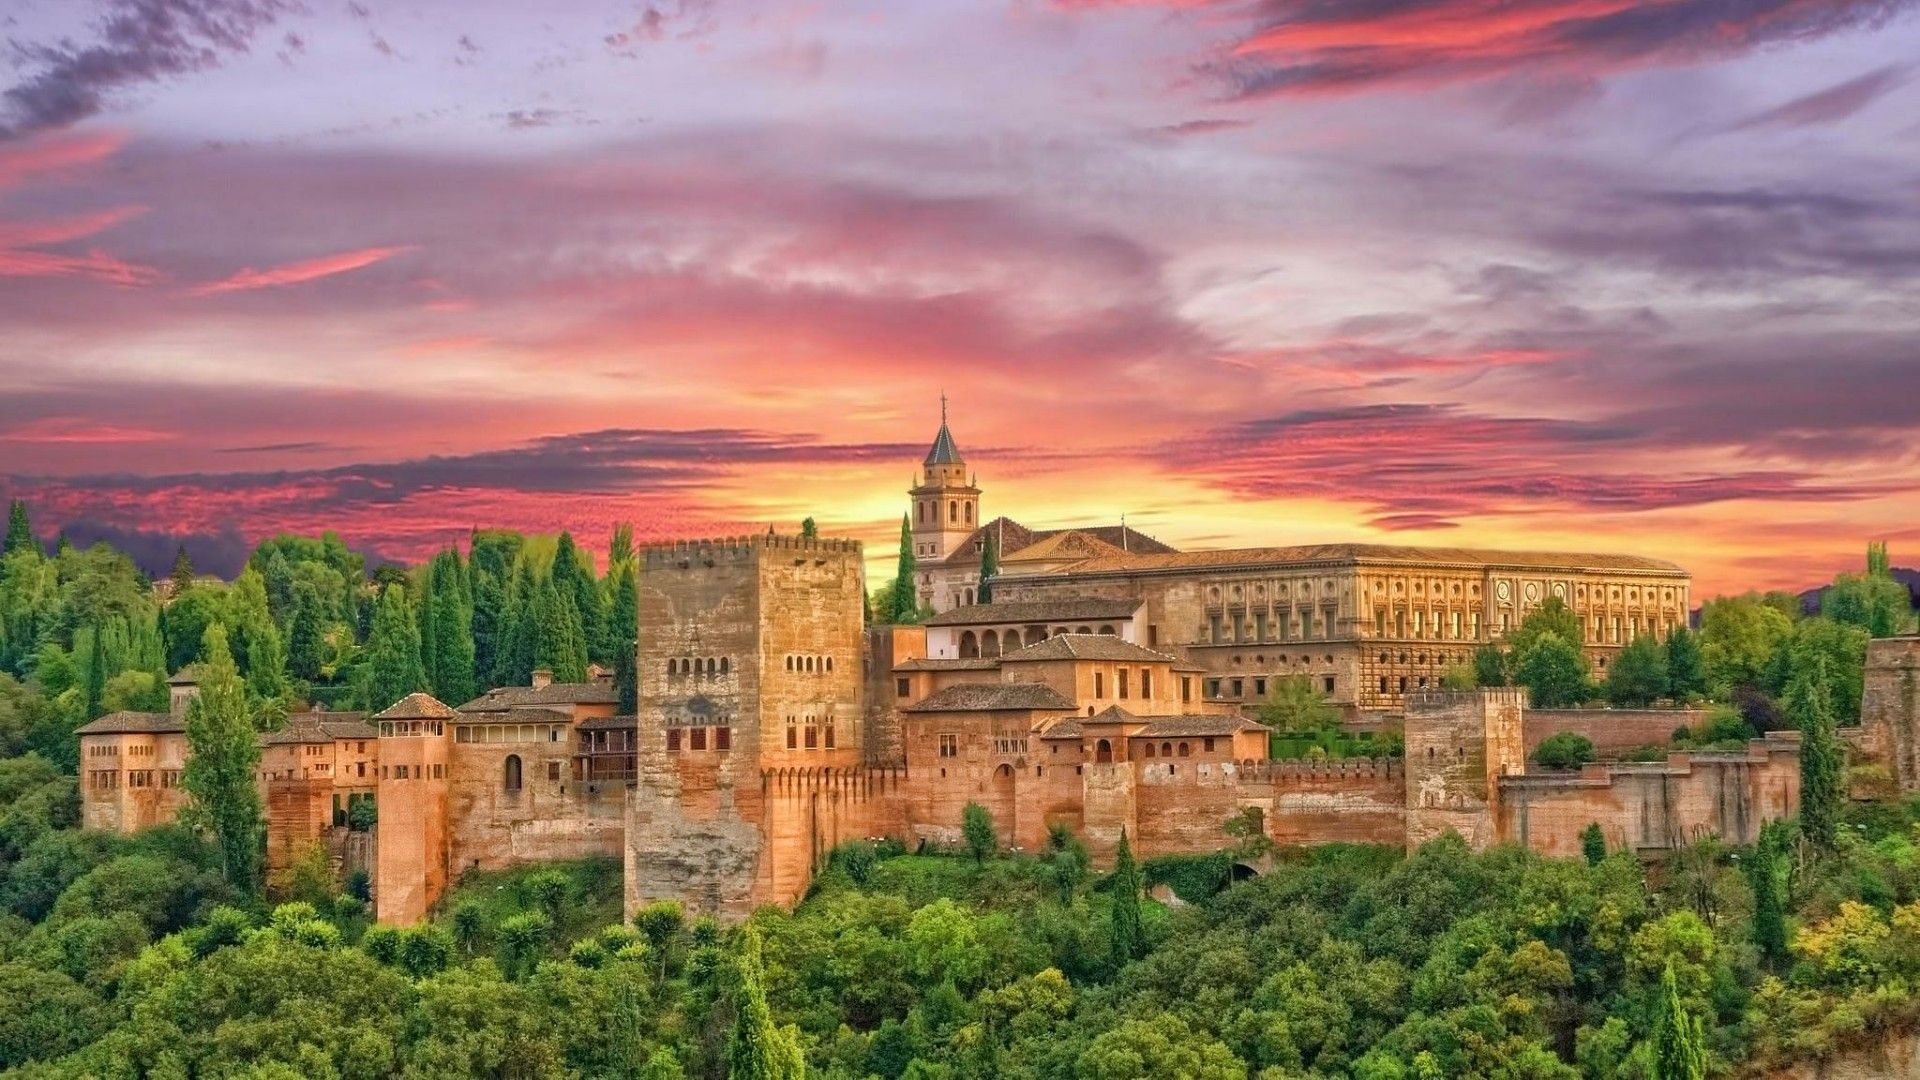
\includegraphics[width=\paperwidth,height=\paperheight,keepaspectratio]{images/granada.jpg}}
}

% Inicio del documento
\begin{document}

% Portada
\maketitle
\thispagestyle{empty}

\begin{center}
    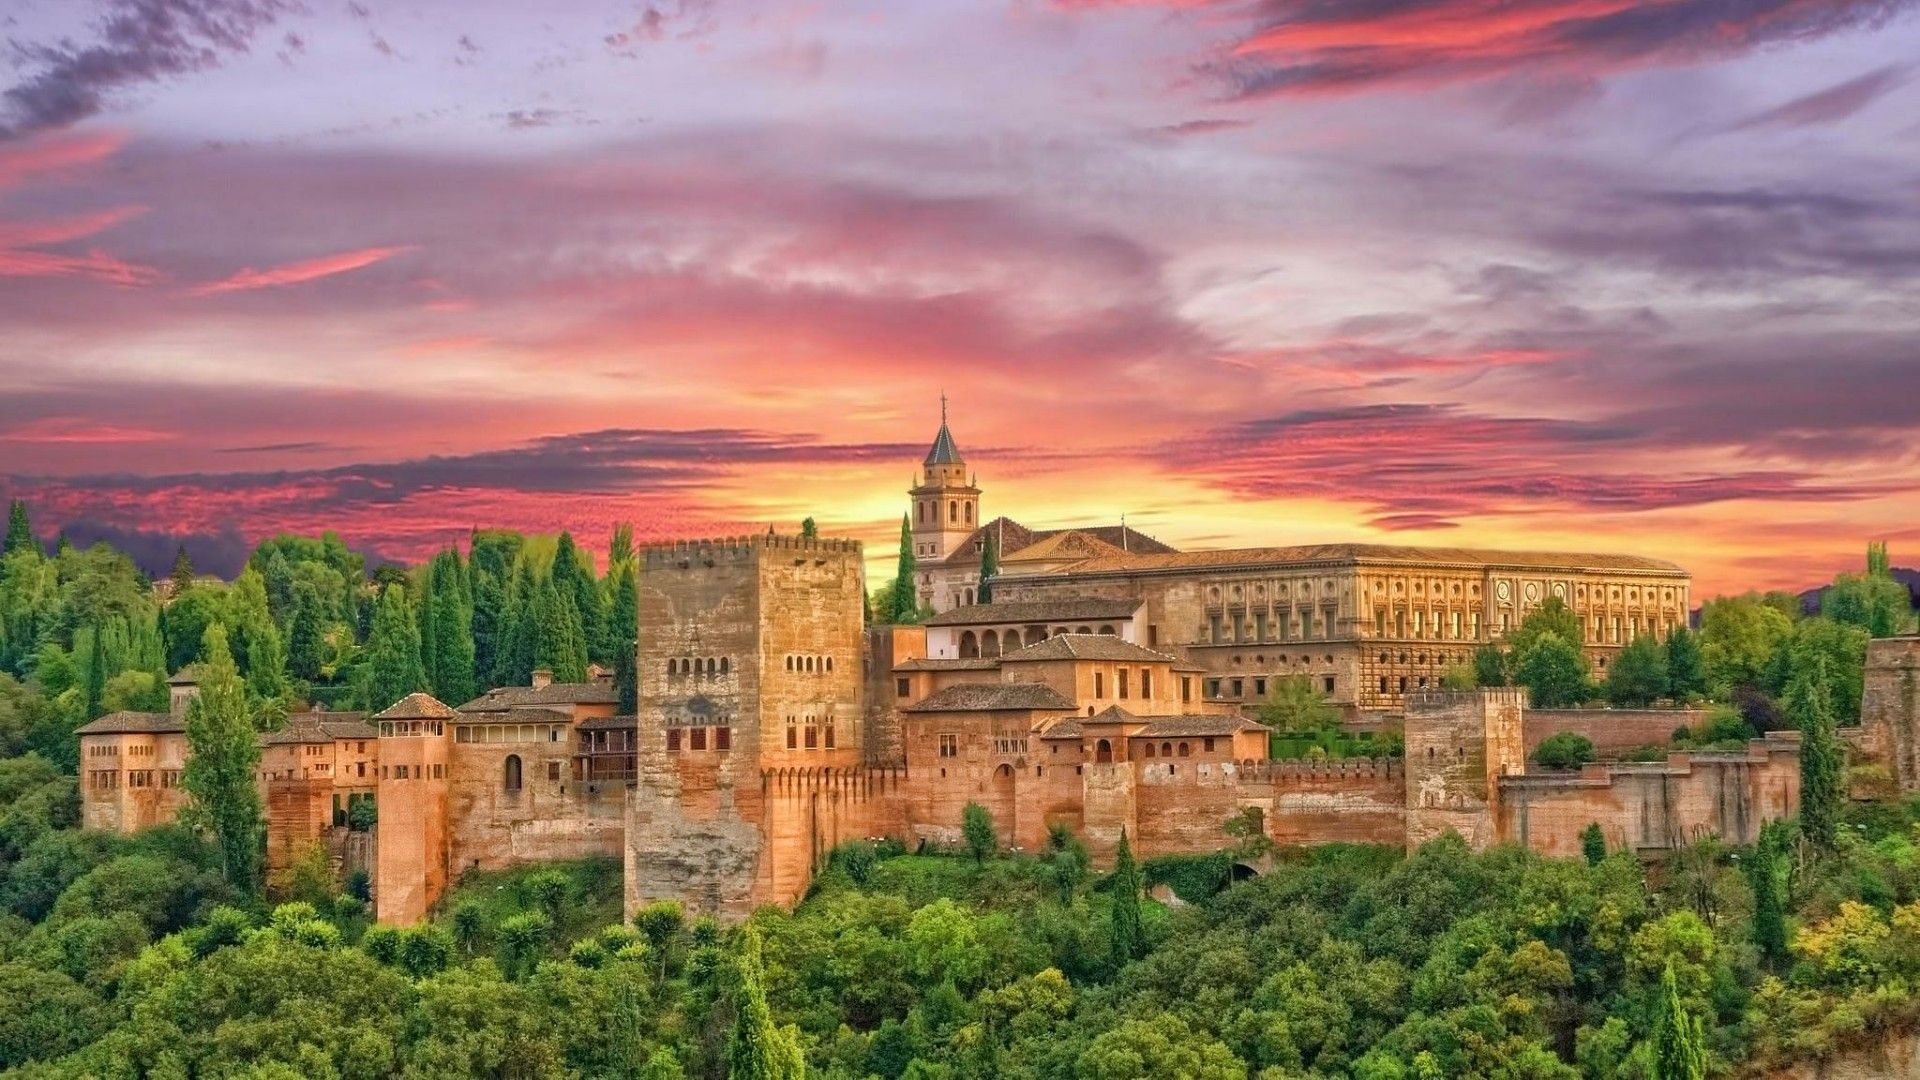
\includegraphics[width=\textwidth,height=0.4\textheight,keepaspectratio]{images/granada.jpg} \\ % Añade tu imagen de fondo
    \vfill
\end{center}

\newpage

% Índice (opcional)
\tableofcontents
\newpage

\section{Concepto y características del inmovilizado intangible}

Es un activo identificable de carácter no monetario y sin apariencia física, además debe de implicar identificabilidad, control sobre el recurso en cuestión y existencia de beneficios futuros.\\

Las inmovilizaciones intagibles son activos no monetarios sin apariencia física, susceptibles de valoriación económica, así como los anticipos a cuenta entregados a proveedores de estos inmovilizados.\\

Podemos concluir que un inmovilizado intangible es un activo identificable, de carácter no monetario y sin apariencia física, cuya proyección económica futura, generalmente por un período superior a un año, se manifiesta en su capacidad para generar flujos positivos de efectivo ya sea mediante la obtención de ingresos o la reducción de costes.\\

\subsection{Características}
\begin{itemize}
    \item inmaterial, sin sustancia física.
    \item controlados económicamente por la empresa.
    \item susceptibles de valoriación económica.
    \item resultado de sucesos pasados.
    \item generar beneficios futuros.
    \item largo personalizado.
    \item pueden sufrir deterioros de valor.
\end{itemize}

\subsection{Inmovilizaciones intangibles}
\begin{itemize}
        \item 200. «Investigación»
        \item 201. «Desarrollo»
        \item 202. «Concesiones Administrativas»
        \item 203. «Propiedad Industrial»
        \item 204. «Fondo de Comercio»
        \item 205. «Derechos de traspaso»
        \item 206. «Aplicaciones Informáticas»
        \item 209. «Anticipos para inmovilizaciones intangibles»
\end{itemize}

\section{Criterios específicos de reconocimento y valoriación}
\subsection{Registro del inmovilizado intangible}
Es preciso que además de cumplir con la definición de activo y los criterios de registro contenidos en el Marco Conceptual, cumpla con la característica de \textit{identificabilidad}, es decir, que sea separable del resto de activos de la empresa.\\

Deben de cumplirse las dos siguientes condiciones:
\begin{itemize}
    \item sea separabe, susceptible de ser separado de la empresa y vendido, entregado para su explotación o intercambiado.
    \item Surja de derechos legales o contractuales con independencia de que tales derechos sean  transferibles o separables de la empresa o de otros derechos y obligaciones.
\end{itemize}

No son inmovilizados intangibles:
\begin{itemize}
    \item Los gastos de establecimiento.
    \item Los gastos de formación.
    \item La publicidad y actividades de propaganda.
    \item Gastos de traslado o reorganización de la empresa.
    \item Elementos generados internamente (p.ej. ni las marcas, cabeceras de periódicos o revistas, sellos o denominaciones editoriales, listas de clientes, etc. que se hayan generado internamente).
\end{itemize}


\subsection{Valoración Inicial}
Es la determinación del precio de coste/adquisición de producción añadiendo los gastos adicionales para de esta manera aprovechar en mayor medida la generación de recursos por parte de la empresa.\\

Además, habrá que sumar los gastos de los impuestos indirectos NO recuperables de la Hacienda Pública, obligaciones de pago futuras por la posesión de dicho activo, así como los gastos financieros devengados.\\

\section{Valoración Posterior}
Todos los activos intangibles tienen en cualquier caso, vida útil definida, considerándose 10 años en el caso de que no se defina.\\

Hay dos tipologías distintas de intangibles. Por un lado, los que tienen vida útil definida y por otro, los que no la tienen.\\

Los inmovilizados intangibles son activos de vida útil definida y, por lo tanto, deberán ser objeto de amortización sistemática en el periódo en el que se prevé que se obtendrán los beneficios económicos futuros derivados de su utilización.\\

Cuando la vida útil de un inmovilizado intangible no pueda ser estimada de forma fiable, se amortizará en un plazo máximo de 10 años.\\

En todo caso, al menos cada año, deberá de comprobarse la existencia de deterioro en el valor de los inmovilizados intangibles, y si es así, se deberá de reconocer la pérdida por deterioro. Este proceso se realizará como llevamos viendo comparando los valores contables con los valores recuperables.\\

Hay algunos elementos cuyo deterioro no puede revertirse como es el caso del \textit{fondo de comercio}, por lo que en estos casos, la pérdida por deterioro se reconocerá directamente en la cuenta de pérdidas y ganancias.\\


\section{Normas Particulares sobre el inmovilizado intangible}

\subsection{Investigación y Desarrollo}
\begin{itemize}
    \item Investigación
\begin{itemize}
    \item Persigue descubrir nuevos conocimientos científicos o técnicos.
    \item No se puede identificar con un proyecto concreto.
\end{itemize}
\item Desarrollo
\begin{itemize}
    \item Es la creación de nuevos productos o servicios.
    \item No se puede identificar con un proyecto concreto.
\end{itemize}

\end{itemize}

Junto a estos se suele incluir \textit{la innovación}, que es la introducción de nuevos productos o servicios en el mercado.\\

\subsubsection{Contabilización}
Para su contabilización debemos de seguir los siguientes pasos:
\begin{enumerate}
    \item Identificación y separación de la fase de investigación de la fase de desarrollo.
    \item Los gastos de investigación serán gastos de ejercicio, aunque la empresa puede activarlos como inmovilizado intangible si cumple con los requisitos:
    \begin{itemize}
        \item Estar individualizados.
        \item Coste claramente establecido.
        \item Motivos fundados por éxito técnico y rentabilidad económica.
    \end{itemize}
    \item Los gastos de desarrollo se reconocerán en el activo y deberán de amortizarse durante su vida útil, \textit{que no puede ser superior a 5 años}.
\end{enumerate}

\textbf{Datos de la práctica:
}\begin{itemize}
    \item Para la contrapartida de la cuenta 200 Investigación, usamos la cuenta 730 Trabajos realizados para el inmovilizado intangible.
    \item Cuando realizamos la amortización, en el caso de la Investigación, debemos de usar la cuenta 2800 Amortización acumulada de Investigación.
    \item En el caso del Desarrollo, usaremos la cuenta 2801 Amortización acumulada de Desarrollo y como cuenta de contrapartida en el activo usaremos la cuenta 6811 Amortización de Gastos de Desarrollo.
    \item ¿Qué entendemos por Propiedad Industrial? Son los derechos de propiedad industrial, como las patentes, marcas, etc.
    \item Cuando se producen pérdidas debemos de usar la cuenta 670 Pérdidas Procedentes del inmovilizado intangible.
\end{itemize}

\subsection{Propiedad Industrial}

\subsubsection{Concepto} 
Se trata de los gastos de desarrollo capitalizados cuando se obtenga la patente, incluido el coste de registro y formalización de la propiedad industrial. También pueden contabilizarse importes por razón de adquisición a terceros.\\

Deben de ser objetos de amortización y de deterioro.\\
Por lo qur:
\begin{itemize}
    \item Vida útil definida, donde se prevé que aportará beneficios a la empresa.
    \item Vida útil definida, se pondrá como máximo el plazo de 10 años.
\end{itemize}

\begin{tcolorbox}[colback=green!5!white,colframe=green!75!black, title=Aclaración]
    Patente = Propiedad Industrial
\end{tcolorbox}

\begin{tcolorbox}[colback=green!5!white,colframe=blue!75!black, title=Nota]
Ejemplo 4 del libro es interesante.
\end{tcolorbox}

\subsection{Concesiones Administrativas}
\subsubsection{Concepto}
Mecanismo contractual utilizado por el Estado o entidad de Derecho Público.\\

El organismo cedente transmite a la empresa concesionaria el derecho y la obligación de gestión de un servicio público durante el período que se establece.\\

Cuando la concesión finaliza hay que entregarlo a la Administración Pública(\textit{concedente}). Dichos activos se amortizarán durante la vida útil de la concesión.\\

\begin{tcolorbox}[colback=yellow!5!white,colframe=yellow!75!black, title=Nota]
\begin{itemize}
    \item ¿Qué es un \textit{canon} que se paga al ayuntamiento? Es un pago que se realiza por el uso de un bien público.
\end{itemize}
\end{tcolorbox}


\subsection{Aplicaciones Informáticas}

\begin{itemize}
\item Se amortizan en un plazo de 5 años salvo prueba en contrario.\\

\item Se deben de aplicar las respectivas amortizaciones y deterioros.\\

\item  En la \textit{práctica} podemos recibir anticipos, anotándolo en la cuente \textit{209 Anticipos para inmovilizaciones intangibles.}

\item A la hora de contabilizar no olvidar el \textit{IVA}.
\end{itemize}


\subsection{Derechos de Traspaso}

Consiste en la cesión mediante un precio de un local de negocio hecha por el arrendatario a un tercero, el cual queda subrogado/sustituido en los derechos y obligaciones del contrato de arrendamiento.\\

Solo pográ figurar en el activo cuando su valor se ponga de mannifiesto en virtud de adquisición onerosa, siendo objeto de amortización y deterioro.\\

Las \textit{reformas} se registrarán como Inmovilizado Material.

\subsection{Fondo de Comercio}

\begin{tcolorbox}[colback=green!5!white,colframe=green!75!black, title=Aclaración]
    ¿Qué es un adquisición onerosa? Es aquella que se realiza mediante un precio.
\end{tcolorbox}

En la adquisición de un negocio por parte de la empresa, el PGC especifica que los elementos se incorporarán por su valor razonable en el momento de adquisición. La valoración de los elementos incorporados puede diferir del precio acordado. Dicha diferencia estaría justificada por las circunstancias que aportan valor al negocio, pero no se pueden contabilizar de manera individual. Este conjunto de elementos es lo que se conoce como \textit{fondo de comercio}.\\

\begin{tcolorbox}[colback=yellow!5!white,colframe=yellow!75!black, title=Fondo de Comercio]
    El fondo de comercio es un concepto contable que representa el valor intangible de una empresa que no puede atribuirse a activos físicos específicos. Este valor intangible puede incluir factores como la reputación de la empresa, la clientela, la marca, las relaciones con los clientes y proveedores, y otros elementos que contribuyen al éxito y la rentabilidad de la empresa.\\

    En términos contables, el fondo de comercio se reconoce cuando una empresa adquiere otra empresa y paga un precio superior al valor razonable de los activos netos identificables adquiridos. \textit{La diferencia entre el precio de compra y el valor razonable de los activos netos se registra como fondo de comercio} en el balance de la empresa adquirente.\\

    El fondo de comercio se amortiza o se somete a pruebas de deterioro periódicamente para reflejar cualquier disminución en su valor.\\

    La vida útil se determinará de manera separada por cada unidad generadora de efectivo.
\end{tcolorbox}


\section{El Inmovilizado Intangible en la cuentas anuales}
Pincha \href{https://github.com/ElblogdeIsmael/ElblogdeIsmael.github.io/blob/main/Asignaturas/Tercer%20A%C3%B1o/CF1/Resumenes/Tema6/ultimaParteT6TeoriaCF1.pdf}{aquí} para ver la última parte del resumen.


\section{Cuestionario tipo test}
Para realizar el tipo test del libro pinche \href{https://elblogdeismael.github.io/Asignaturas/Tercer%20A%C3%B1o/CF1/Tests/testT6Libro.html}{aquí.}

\end{document}

